\chapter{Membrane-Associated Enzymes}
\setlength{\headheight}{12.71342pt}
\addtolength{\topmargin}{-0.71342pt}

\section{Introduction}  
Many enzymes have been identified in milk fat globules (MFGs) and extracellular vesicles (EVs), with advancements in proteomic techniques continuously expanding this knowledge. However, many of these enzymes are present in low abundance and often originate from endoplasmic reticulum (ER), Golgi membranes, or cytosolic remnants. A large proportion remains inactive in milk due to the absence of relevant substrates or a suitable environment. This chapter focuses on sulfhydryl oxidase, catalase, lactoperoxidase (LPO), xanthine oxidoreductase (XOR), $\gamma$-glutamyltransferase (GGT), and 5'-nucleotidase, discussing their relevance in mammary gland biology, milk integrity, and physiological function upon consumption \cite*{RM_01}.  

\section{Classification of Mechanisms of Enzymes}
Sulfhydryl Oxidase (EC 1.8.3.2) is an enzyme that helps form chemical bindings in proteins by catalysing the oxidation of protein thiols (SH-groups) to form disulphides (-S-S-) while simultaneously reducing oxygen to hydrogen peroxide. In milk, both metal-dependent and flavin-dependent sulfhydryl oxidase types have been identified, where the flavin-dependent sulfhydryl oxidase is the most common in bovine milk \cite*{RM_01}.

\vline

Catalase (EC 1.11.1.6) is an enzyme found in almost all living organisms exposed to oxygen. It catalyses hydrogen peroxide to water and oxygen.

\begin{equation}
    2 H_2O_2 \rightarrow 2 H_2O + O_2
    \label{eq_01}    
\end{equation}

From the given material, it has not been possible to detect catalase in milk \ref*{fig_01}. When catalase is detected in milk, it is due to somatic cells or contamination, such as when the cow has mastitis \cite*{RM_01}.

\begin{figure}[h]
    \centering
    \includegraphics*[width=0.8\linewidth]{Figures/table_01.png}
    \caption{Table 6.1 from the book with the selected enzymes in the chapter \cite*{RM_01}.}
    \label{fig_01}
\end{figure}

\vline 

Lactoperoxidase (EC 1.11.1.7) is a heme containing peroxidase enzyme. Found in large quantities in bovine milk (30mg/L) where it functions as an antimicrobial defence by oxidizing thiocyanate to hypothiocyanite (se formlen). That is why the amount of lactoperoxidase is higher if the if the cow has mastitis. Has an antimicrobial activity against both Gram-positive and Gram-negative bacteria. When it bounds to calcium it is very heat stable up to 80\textdegree C \cite*{RM_01}. Oxidation of thiocyanate to hypothiocyanite can be seen in equation \ref*{eq_02}.

\begin{equation}
    H_2O_2 + SCN^- \rightarrow H_2O + OSCN^-
    \label{eq_02}
\end{equation}

\vline 

Xanthine Oxidoreductase (XOR) (EC 1.17.3.2) is an enzyme that has been identified in both skim milk and cream phospholipid membranes. It is released from the Milk Fat Globule Membrane (MFGM) during phase inversion. Significant amounts can be removed through washing with non-ionic detergents or high salt concentrations. XOR is classified as a peripherally associated membrane protein with both soluble and insoluble properties, due to its ability to associate with membranes while also being extractable under certain conditions. It has been detected in extracellular vesicles (EVs) and MFGs in both human and bovine milk. Proteomic studies have further confirmed the presence of XOR in extracellular vesicles (EVs) and milk fat globules (MFGs) in both human and bovine milk \cite*{RM_01}.

\vline

$\gamma$-Glutamyltransferase (EC 2.3.2.2) Catalyzes transfer of $\gamma$-glutamyl groups from glutathione to amino acids, peptides, or water. Found in cell membranes and  has been suggested to aid amino acid supply for milk protein synthesis. Primarily located in skim milk rather than MFGM (74.3\% vs 6.6\%) \cite*{RM_01}.

\section{Role of Enzymes in Milk and Dairy Products}

In the following section, we will briefly discuss the effects of membrane-associated enzymes on milk and dairy products, focusing on their role in protein modification and lipid metabolism through oxidative reactions \cite{RM_01}.

\vline

Sulfhydryl 

\section{Summary of Recent Scientific Studies}
To limit the scope of this report, it was decided to investigate one enzyme from the given literature \cite*{RM_01}. Lactoperoxidase was selected due to its antimicrobial properties and a relevant scientific study by Aouadhi et al. (2024) was identified and used in current section. 

\vline

Lactoperoxidase (LPO) combined with hydrogen peroxide and thiocyanate forms a well described system called the Lactoperoxidase System (LPS), known for its antimicrobial properties through production of hypothiocyanite which impairs protein functions in organisms like E. coli, yeasts, and molds \cite*{RM_02}

\vline

A recent study by Aouadhi et al. (2024) investigated the impact of combining the LPS system with nisin and/or heat treatment to enhance the microbial safety and shelf life of raw milk products through decrease of microbial load. 
Nisin was chosen as it increases membrane permeability thereby facilitate transport of hypothiocyanite through membranes to impair cellular proteins. In contrast, heat treatment reduces the initial microbial load, enhancing the system's efficacy.

\vline

As noted in \cite*{RM_01}, the LPS system remains inactive in bovine milk due to low concentrations of hydrogen peroxide and thiocyanate. Aouadhi et al. (2024) confirmed this and activated the system by adding hydrogen peroxide and thiocyanate to the raw milk. Following activation, nisin was added in different concentrations, and samples were incubated at 25\textdegree C for 72 hours. Microbial analysis following the experiment revealed:
\begin{itemize}
    \item 6-log reduction in total mesophilic bacteria
    \item 5-log reduction in coliforms
    \item 4-log reduction in yeasts and molds
\end{itemize}


These reductions were achieved with 7 mg/L SCN, 15 mg/L hydrogen peroxide, and 50 IU/mL nisin after 72 hours of incubation at 25\textdegree C. 

\vline 

With the optimal concentrations an experiment was prepared including pasteurization. The LPS system was activated for 2, 4 and 6 hours before pasteurization at 63\textdegree C for 30 minutes and subsequent incubation at 4\textdegree C and 25\textdegree C for 96 hours. All samples were analyzed for total bacterial count, coliforms, yeasts and mold. Results for coliforms are shown below in figure \ref*{fig_02}:

\begin{figure}[h]
    \center
    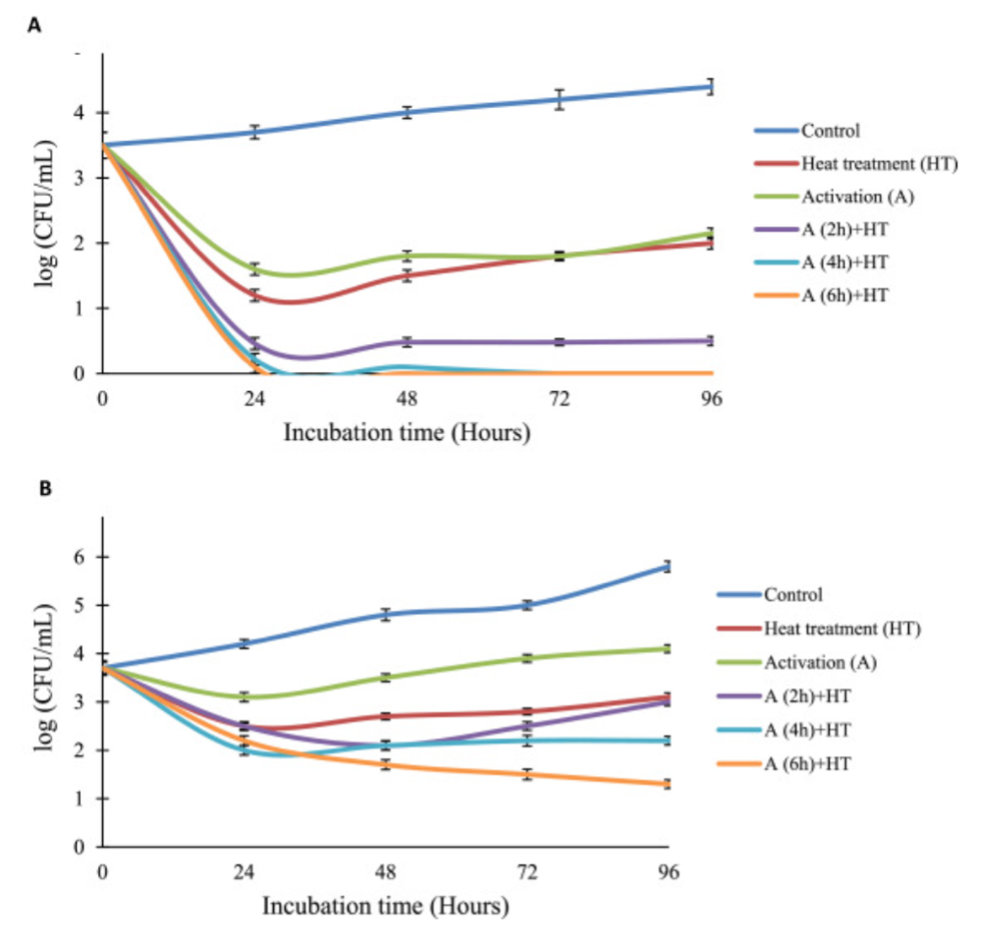
\includegraphics[width=0.8\linewidth]{Figures/fig_01.png}
    \caption{Evolution of total coliforms in raw cow milk according to different treatments at 4\textdegree C (A) and 25\textdegree C (B) for 96 h \cite{RM_02}}
    \label{fig_02}
\end{figure}

From \ref*{fig_01}, it is evident how the concentration of coliforms steadily increases in the control sample, incubated without any treatment. In contrast, the heat-treated sample show an initial decrease in coliforms, followed by an increase after 24 hours of incubation at both temperatures (4\textdegree C and 25\textdegree C). Samples where LPS was activated before heat treatment shows the greatest log reduction in coliforms when stored at 4\textdegree C for 96 hours. Although a significant reduction is also observed at 25\textdegree C, the effect is less pronounced compared to storage at 4\textdegree C, highlighting the impact from incubation temperature on microbial growth.

\vline

Identical results were obtained for yeasts, and molds with complete destruction at 4\textdegree C with 4 and 6-hour LPS activation before heat treatment. 

\vline

The article concludes that LPS activation cycles of 4 and 6 hours before heat treatment (pasteurization) show promising results in reducing the microbial load of milk and thereby the quality. This while utilizing an already present enzyme in milk, LPO, combined with a food grade approved preservative nisin.

\section{Conclusion}
